\chapter{Эксперимент Belle} \label{sec:belle-exp}
\section{Ускоритель KEKB} \label{sec:kekb}
Ускоритель \kekb --- это асимметричный \ep-коллайдер с энергией в \cms $\sqrt{s}=10.58\gev$, соответствующей массе резонанса~\ups, разработанный для рождения большого количества \bbbar-пар.  Ускоритель введен в эксплуатацию в 1998 году и состоит из двух накопительных колец периметром примерно $3~\textrm{км}$, находящихся в $11\textrm{м}$ под землей (рисунок~\ref{fig:KEKB}).  Электроны и позитроны ускоряются до энергий $8\gev$ и $3.5\gev$, соответственно.  Пучки электронов и позитронов циркулируют в соответствующих накопительных кольцах и пересекаются в единственном месте взаимодействия под углом $11~\textrm{мрад}$.
\begin{figure}[htb]
 \centering
  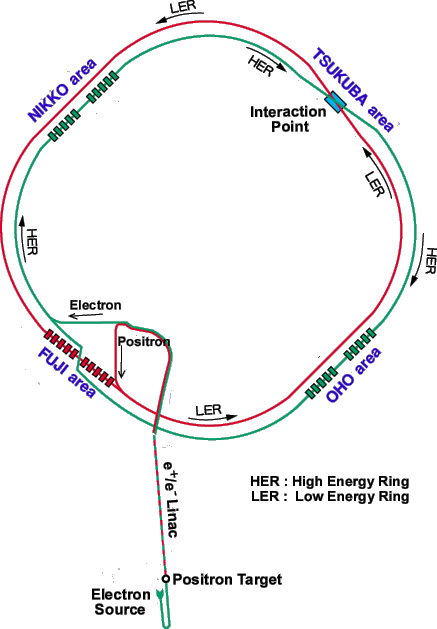
\includegraphics[width=0.5\textwidth]{KEKB}
  \caption{Ускоритель \kekb.}
\label{fig:KEKB}
\end{figure}

Разность энергий пучков ускорителя \kekb соответствует Лоренц-фактору $\bg_{\ups}=0.425$ в лабораторной системе отсчета.  Начальный импульс $B$-мезонов приводит к доступному для измерения пространственному разделению вершин распада двух рожденных $B$-мезонов, равному примерно $200\mum$. При симметричном рождении пространственное разделение составляло бы примерно $30\mum$.

Ускоритель \kekb разрабатывался для достижения светимости $\mcl=1.0\times 10^{34}\lumi$, соответствующей рождению десяти \bbbar-пар в секунду.  В течение работы, ускоритель был существенно модернизирован.  В частности, оснащен технологией crab cavities, увеличивающий светимость за счет поворота пучков в вблизи области взаимодействия.  Эти усилия позволили превзойти многие заложенные при проектировании параметры, достичь рекордной светимости $\mcl=2.1\times 10^{34}\lumi$.

Детектор \belle набрал интеграл светимости $711\ifb$, соответствующий $772\times10^6$ \bbbar-парам, рожденным на ускорителе \kekb, работающем вблизи резонанса \ups.  Кроме того, ускоритель \kekb работал при других энергиях.  В частности, детектор Belle набрал интеграл светимости $121\ifb$ на резонансе $\Upsilon(5S)$, что позволяет проводить измерения в системе $B_s$-мезонов, а также изучать спектроскопию $b\overline{b}$-состояний.  Полный интеграл светимости, набранный детектором Belle на ускорителе \kekb превышает~$1~\textrm{абн}^{-1}$ (рисунок~\ref{fig:KEKB-lum}).

\begin{figure}[htb]
 \centering
  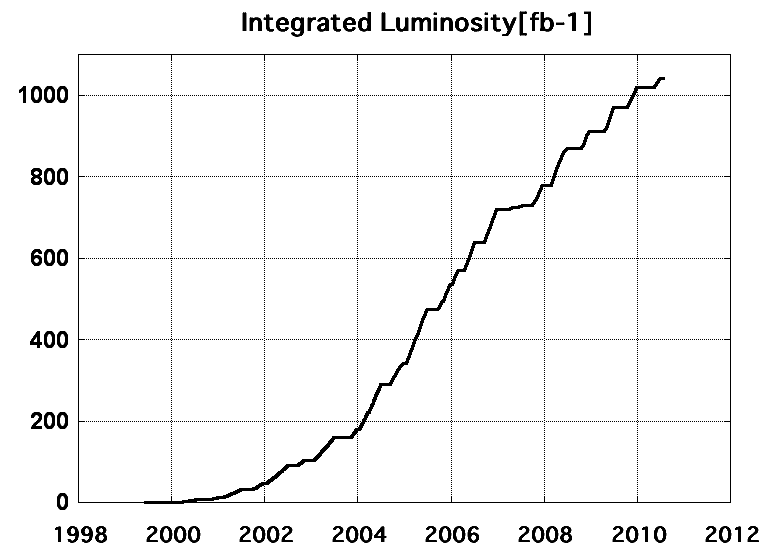
\includegraphics[width=0.5\textwidth]{KEKB-luminosity-bw.png}
  \caption{Интеграл светимости, набранный детектором \belle на ускорителе \kekb.}
\label{fig:KEKB-lum}
\end{figure}

Детальное описание ускорителя \kekb приведено в работах~\cite{KEKB1,KEKB2}.

\clearpage
\section{Детектор Belle}\label{sec:belle}
Детектор $\belle$ --- это универсальный детектор, охватывающий близкий к $4\pi$ телесный угол вокруг области взаимодействия пучков.  Детектор оптимизирован для выполнения времязависимых  измерений и работе с асимметричным \ep-коллайдером \kekb.  Схема детектора приведена на рисунке~\ref{fig:Belle}.  

\begin{figure}[htb]
 \centering
  \includegraphics[width=\textwidth]{BelleDetector}
  \caption{Детектор \belle.}
\label{fig:Belle}
\end{figure}

Детектор \belle оборудован сверхпроводящим магнитом, создающим магнитное поле $1.5~\textrm{Тл}$, и несколькими подсистемами для регистрации и идентификации заряженных и нейтральных частиц.  Треки заряженных частиц реконструируются на основе измерений кремниевого вершинного детектора (\svd) и центральной дрейфовой камеры (\cdc).  Электромагнитные ливни регистрируются кристаллами \csit электромагнитного калориметра (\ecl).  Кристаллы \textrm{BGO} переднего калориметра малых углов закрывают трубу ускорителя, уменьшая фон для \cdc, и используются в качестве монитора светимости.  Мюоны и $K_L^0$-мезоны регистрируются счетчиками, помещенными в железное ярмо, замыкающее магнитный поток.  Помимо измерения потери энергии в \cdc, идентификация частиц производится с помощью измерений аэрогелевых пороговых черенковских счетчиков и времяпролетных счетчиков, расположенных за пределами \cdc.



Расположение и принципы работы некоторых подсистем детектора \belle кратко описаны в следующих пунктах.  Описания следуют техническим публикациям, ссылки на которые приведены, и в которых может быть найдена более полная информация.  Для анализа данных с детектора \belle, описанного в главе~\ref{sec:bdsth}, важны: трековая система, электромагнитный калориметр и системы идентификации частиц.

%\subsection{Труба ускорителя}\label{sec:beam-pipe}
\subsection{Кремниевый вершинный детектор}\label{sec:svd}
Основной целью эксперимента \belle является наблюдение времязависимого нарушения \cpconj-нарушения в распадах нейтральных $B$-мезонов.  Для таких анализов необходимо прецизионное измерение расстояния между вершинами распадов двух $B$-мезонов, рожденных при распаде резонанса \ups.  В разделе~\ref{sec:kekb} обсуждалось, что характерное расстояние между вершинами составляет примерно $200\mum$.  Необходимо, таким образом, чтобы кремниевый вершинный детектор (\svd) обладал высоким пространственным разрешением и был способен определить $z$-координату трека с точностью около $100\mum$.

\svd является ближайшим к области взаимодействия пучков детектором.  Он расположен вблизи бериллиевой трубы ускорителя.  Этот детектор должен быть устойчив к большим дозам облучения, обусловленным пучковым фоном.  \svd разделен на слои различных радиусов вокруг трубы ускорителя.  В каждом слое установлены пластины двусторонних кремниевых полосковых детекторов (\dssd).  \dssd содержат обедненные $pn$-переходы.  Проходя сквозь обедненные $pn$-переходы, заряженные частицы создают электрон-дырочные пары вдоль своей траектории.  Электроны и дырки дрейфуют, соответственно, к $n$- и $p$-полоскам на поверхности \dssd.  $n$-полоски расположены перпендикулярно, а $p$-полоски расположены вдоль оси пучков.  Таким образом обеспечивается измерение координат траектории вдоль направлений $r\varphi$ и $z$, соответственно.

Два разных вершинных детектора работали в эксперименте \belle.  Первоначальный \svd, который мы будем называть $\svd1$, работал с $1999$ по $2003$ годы.  Детектор $\svd1$ имеет цилиндрическую структуру и состоит из трех слоев с радиусами $30\mm$, $45.5\mm$ и $60.5\mm$.  Он охватывает диапазон полярных углов от $23\grad$ до $139\grad$, что соответствует $86\%$ полного телесного угла.  $\svd1$ состоит из $102$ \dssd.  Каждый \dssd имеет $1280$ чувствительных полосок и по $640$ считывающих каналов на противоположных сторонах.  Пространственный период полосок составляет $42\mum$ в направлении $z$ и $25\mum$ в направлении $\varphi$.  Площадь активной зоны \dssd составляет приблизительно $55\times 33\mm^{2}$.

\svd был модернизирован в $2003$ году.  Модернизированную версию \svd мы будем называть $\svd2$.  $\svd2$ расположен ближе к трубе ускорителя и покрывает больший диапазон полярных углов $\theta$.  Расположение частей $\svd2$ показано на рисунке~\ref{fig:svd}.  Он состоит из четырех слоев радиусами $20\mm$, $43.5\mm$, $70\mm$ и $88\mm$ и покрывает диапазон полярных углов от $17\grad$ до $150\grad$, что соответствует $93\%$ полного телесного угла.  $\svd2$ состоит из $246$ \dssd.  Используются два типа \dssd с пространственным периодом полосок от $50\mum$ до $75\mum$.  Площадь активно зоны \dssd в первых трех слоях составляет $28.4\times 79.6\mm^{2}$, а в четвертом слое --- $34.9\times 76.4\mm^{2}$.

% \begin{figure}[H]
%  \centering
%  \begin{minipage}{0.49\textwidth}
%  \centering
%  \vspace{0.9 cm}
%   \includegraphics[width=0.7\textwidth]{svd1}
%   \subcaption{}
%   \label{fig:svd1}
%  \end{minipage}
%  \begin{minipage}{0.49\textwidth}
%   \centering
%   \includegraphics[width=0.9\textwidth]{svd2}
%   \subcaption{}
%   \label{fig:svd2}
%  \end{minipage}
%   \\
%   \begin{minipage}{0.8\textwidth}
%   \includegraphics[width=\textwidth]{svd_front_v2}
%   \subcaption{}
%   \label{fig:svd2-front}
%  \end{minipage}
%   \caption{Расположение чувствительных полосок а) $\svd1$ и б) $\svd2$ и в) схема расположения $\svd2$.}
% \label{fig:svd}
% \end{figure}

Количественной характеристикой работы \svd является разрешение при измерении прицельного параметра трека.  Прицельным параметром заряженного трека называется наименьшее расстояние до точки взаимодействия пучков.  Разрешение при измерении прицельного параметра может отличаться для \rphi- и $z$-направлений, а также может зависеть от импульса и полярного угла $\theta$ частицы.  Разрешение в \rphi- и $z$-направлениях может быть описано следующими функциями:
\begin{equation}
\begin{split}
 &\sigma^{1}_{\rphi} = 19.2\mum \oplus \frac{54.0\mum}{p\beta\sin^{3/2}\theta},\quad
  \sigma^{1}_{z}     = 42.2\mum \oplus \frac{44.3\mum}{p\beta\sin^{5/2}\theta},\\
 &\sigma^{2}_{\rphi} = 21.9\mum \oplus \frac{35.5\mum}{p\beta\sin^{3/2}\theta},\quad
  \sigma^{2}_{z}     = 27.8\mum \oplus \frac{31.9\mum}{p\beta\sin^{5/2}\theta}, 
\end{split}
\end{equation}
где символ $\oplus$ обозначает квадратичное сложение, индексы $1$ и $2$ соответствуют $\svd1$ и $\svd2$ и импульс $p$ выражен в\gevc (смотрите рисунок~\ref{fig:svd-resolution}).  Детальное описание \svd приведено в работах~\cite{svd1,svd2}.

\begin{figure}[H]
 \centering
 \begin{minipage}{0.39\textwidth} 
 \begin{subfigure}{\linewidth}
 \centering
  \includegraphics[width=0.7\textwidth]{svd1}
  \subcaption{}
  \label{fig:svd1}
 \end{subfigure}\\ \vspace{0.1 cm}
 
 \begin{subfigure}{\linewidth}
  \centering
  \includegraphics[width=0.9\textwidth]{svd2}
  \subcaption{}
  \label{fig:svd2}
 \end{subfigure}
% \vspace{0.9 cm}
 \end{minipage}
 \begin{minipage}{0.59\textwidth}
  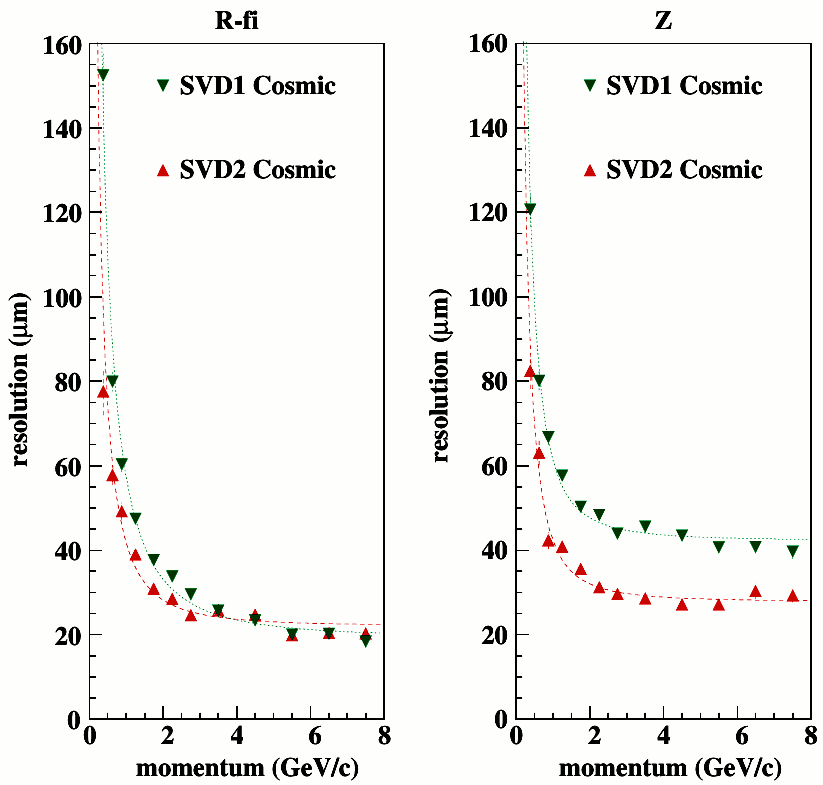
\includegraphics[width=\textwidth]{svd-resolution-16bit}
  \subcaption{}
  \label{fig:svd-resolution}
 \end{minipage}
  \\
  \begin{minipage}{0.8\textwidth}
  \includegraphics[width=\textwidth]{svd_front_v2}
  \subcaption{}
  \label{fig:svd2-front}
 \end{minipage}
  \caption{Схемы расположения чувствительных полосок а)~$\svd1$ и б)~$\svd2$; в)~разрешение по прицельному параметру трека в зависимости от импульса частицы; г)~схема расположения $\svd2$.}
\label{fig:svd}
\end{figure}

% [78] Y. Ushiroda. “Belle Silicon Vertex Detectors”. Nuclear Instruments and Methods A, 511
% (1–2):6–10, 2003. Proceedings of the 11th International Workshop on Vertex Detectors.
% [79] Z. Natkaniec, H. Aihara, Y. Asano et al. “Status of the Belle Silicon Vertex Detector”.
% Nuclear Instruments and Methods A, 560(1):1–4, 2006.
% [80] M. Fujikawa. “Measurement of Branching Fraction and Time-dependent CP Asymme-
% try Parameters in B0 → K0 π0 Decays”. PhD thesis, Nara Women’s University, 2009.

%\subsection{Калориметр малых углов}\label{sec:efc}

\subsection{Центральная дрейфовая камера}\label{sec:cdc}
Центральная дрейфовая камера (\cdc) разработана для реконструкции треков заряженных частиц.  \cdc расположена внутри магнитного поля $1.5~\textrm{Тл}$, создаваемого сверхпроводящим магнитом, что позволяет определять импульс заряженных частиц, используя кривизну восстановленных треков.  Кроме того, \cdc используется для измерения энергетических потерь заряженных частиц ($\dd E/\dd x$), которые используется для идентификации частиц.  Информация от \cdc также используется в системе триггера.

\cdc~--- это цилиндрическая проволочная дрейфовая камера, состоящая из $50$ слоев анодных проволочек и трех слоев катодных полосок.  Длина \cdc составляет $2404\mm$, внутренний и внешний радиусы равны $83\mm$ и $888\mm$.  Расположение \cdc показано на рисунке~\ref{fig:cdc}.  Чтобы учесть асимметрию энергий пучков, \cdc асимметрична в направлении $z$ и покрывает диапазон полярных углов от $17\grad$ до $150\grad$, что соответствует $92\%$ полного телесного угла.  \cdc состоит из $8400$ дрейфовых ячеек, организованных в $6$ аксиальных и $5$ стерео слоев.  Каждый стерео слой содержит от $3$ до $6$ радиальных слоев с одинаковым количеством дрейфовых ячеек в азимутальном направлении.  Дрейфовые ячейки состоят из $8$ проволочек с отрицательным потенциалом, обеспечивающих электрическое поле вокруг проволочки с положительным потенциалом.  Структура ячейки и расположение проволочек показаны на рисунке~\ref{fig:cdc-cell}

\cdc наполнен газовой смесью, состоящей на $50\%$ из гелия и на $50\%$ из этана.  Смесь из газов с небольшой атомной массой $Z$ минимизирует влияние множественного кулоновского рассеяния, особенно для частиц с небольшим импульсом, и уменьшает фон от синхротронного излучения благодаря малости сечения фотоэффекта.  Кроме того, этановая компонента обеспечивает хорошее разрешение по \dedx.

Проходя через дрейфовые ячейки, заряженные частицы ионизируют газ вдоль своей траектории.  Образовавшиеся ионы и свободные электроны дрейфуют, соответственно, к катодным и анодным проволочкам.  В сильном электрическом поле анодных проволочек происходит усиление электрического сигнала, регистрируемого чувствительными проволочками.  Проволочки в аксиальных слоях позволяют измерить поперечный импульс \pt, в то время как стерео слои, установленные с малым углом, дают дополнительную информацию для измерения продольной компоненты импульса \pl.  Детальное описания алгоритма восстановления трека и определения импульса приведено в работе~\cite{cdc}.

\begin{figure}[h]
 \centering
  \includegraphics[angle=270,width=\textwidth]{cdcfig_01}\\
  \caption{Схема расположения центральной дрейфовой камеры детектора \belle~\cite{BelleNIM}.}
\label{fig:cdc}
\end{figure}

\begin{figure}[H]
 \centering
\includegraphics[width=0.35\textwidth]{cdcfig_02}\hfill
\includegraphics[width=0.5\textwidth]{cdcfig_03}
  \caption{Схема расположения проволочек в центральной дрейфовой камере детектора \belle~\cite{BelleNIM}.}
\label{fig:cdc-cell}
\end{figure}

Разрешение по поперечному импульсу в \cdc описывается функцией
\begin{equation}
 \left.\frac{\sigma_{\pt}}{\pt}\right|_{\cdc} = \left(0.28\pt\oplus\frac{0.35}{\beta}\right)\%,
\end{equation}
где $\pt$ обозначает величину поперечного импульса трека в\gevc и $\beta$ обозначает скорость частицы в единицах скорости света.  При комбинировании информации с \cdc и \svd, разрешение по \pt улучшается:
\begin{equation}
 \left.\frac{\sigma_{\pt}}{\pt}\right|_{\cdc+\svd} = \left(0.19\pt\oplus\frac{0.30}{\beta}\right)\%.
\end{equation}

Амплитуды сигналов сработавших проволочек используются для измерения потери энергии (\dedx) заряженной частицы в \cdc.  Величина потерь \dedx подчиняется формуле Блоха и зависит от скорости частицы.  Скорость при данном импульсе зависит от массы частицы и, значит, измерение \dedx может быть использовано для идентификации заряженных частиц.  Измеренные значения \dedx подчиняются распределению Ландау с широкими хвостами, поэтому для оценки наиболее вероятного измеренного значения \dedx применяется метод усеченного среднего, позволяющий минимизировать вклад больших флуктуаций.  Зависимость \dedx от импульса частицы приведена на рисунке~\ref{fig:dedx}.

Детальное описание \cdc содержится в работах~\cite{BelleNIM,cdc}.

\begin{figure}[H]
 \centering
 \includegraphics[width=0.8\textwidth]{cdcfig_dEdx}\\
  \caption{Зависимость ионизационных потерь от импульса частиц.  Точками показаны экспериментальные данные, линиями --- ожидаемые энергетические потери для различных типов частиц~\cite{BelleNIM}.}
\label{fig:dedx}
\end{figure}

%[cdc1] [81] Belle Tracking Group. “Charged Particle Tracking at Belle”. Belle Note #327, 2000.
%[cdc2] [82] H. Hirano, M. Akatsu, Y. Fujita et al. “A High-resolution Cylindrical Drift Chamber for the KEK B-Factory”. Nuclear Instruments and Methods A, 455(2):294–304, 2000.

\subsection{Аэрогелевые черенковские счетчики}
Аэрогелевый черенковский счетчик (\acc) --- это детектор для идентификации частиц, в данном случае для разделения заряженных $\pi$- и $K$-мезонов.  Он обладает разделительной способностью в диапазоне импульсов заряженных частиц от $1\gevc$ до $4\gevc$, расширяя диапазон, в котором применима идентификация по $\dd E/\dd x$ и по информации от времяпролетных счетчиков.

Заряженные частицы, пролетающие сквозь среду со скоростью, превышающей скорость распространения света в этой среде, излучают свет, называемый черенковским излучением.  Условие, при котором возникает черенковское излучение, зависит от показателя преломления среды следующим образом:
\begin{equation}
 n>\frac{1}{\beta}=\sqrt{1+\left(\frac{m}{p}\right)^2},
\end{equation}
где $\beta$ --- скорость частицы и $n$ --- показатель преломления среды.  Материал среды в \acc выбран таким, чтобы $\pi$-мезоны с импульсом больше $1\gevc$ производили черенковское излучение, но чтобы скорость более тяжелых заряженных $K$-мезонов с тем же импульсом была под порогом генерации черенковского излучения.  \acc работает только как пороговый счетчик, не измеряя черенковский угол, зависящий от скорости частицы,  и который также может быть использован для идентификации частиц.

\acc разделен на цилиндрическую и торцевую части, которые покрывают полярный угол от $17\grad$ до $127\grad$.  Цилиндрическая часть детектора состоит из $960$ счетчиков, сгруппированных в $60$ ячеек в $\varphi$-направлении.  Торцевая часть детектора состоит из $228$ счетчиков, сгруппированных в $5$ концентрических слоя.  Счетчики направлены в место встречи пучков.  Расположение счетчиков показано на рисунке~\ref{fig:acc}.  Каждый счетчик состоит из слоя кварцевого аэрогеля, расположенного в алюминиевом корпусе размером $12\times12\times12\cm^{3}$.  Коэффициент преломления кварцевого аэрогеля находится в диапазоне от $1.010$ до $1.030$ и зависит от полярного угла.  Черенковский свет регистрируется сеточными фотоумножителями, закрепленными в алюминиевых корпусах.

Используя только сигналы с \acc, можно идентифицировать заряженные $K$-мезоны с импульсами до $4\gevc$ с эффективностью больше $80\%$ при соответствующей ошибочной $\pi$-мезонной идентификацией меньше $10\%$.

Детальное описание \acc содержится в работах~\cite{BelleNIM,acc}.

\begin{figure}[H]
 \centering
 \includegraphics[width=\textwidth]{ACC_det_clean}\\
  \caption{Расположение аэрогелевых черенковских и времяпролетных счетчиков детектора \belle~\cite{BelleNIM}.}
\label{fig:acc}
\end{figure}

%[acc] [83] T. Iijima, I. Adachi, R. Enomoto et al. “Aerogel Cherenkov Counter for the Belle De-
%tector”. Nuclear Instruments and Methods A, 453(1):321–325, 2000.

\subsection{Времяпролетные счетчики}
Система времяпролетных счетчиков (\tof) измеряет время, за которое частица прошла расстояние от места встречи до \tof.  Сопоставляя результаты измерения с измеренным импульсом, можно получить полезную для идентификации частицы информацию, в частности, для разделения заряженных $\pi$- и $K$-мезонов.  \tof обладают достаточной разрешающей способностью для заряженных частиц с импульсом меньше $1.2\gevc$.  Таким образом, система \tof является комплиментарной к системе \acc.  Кроме  того, система \tof генерирует быстрые временные сигналы для триггерной системы.

\begin{figure}[htb]
 \centering
 \includegraphics[width=\textwidth]{toffig1}\\
  \caption{Расположение времяпролетных счетчиков детектора \belle~\cite{BelleNIM}.}
\label{fig:tof}
\end{figure}

\tof состоят из пластиковых сцинтилляционных пластин, присоединенных к сеточным фотоумножителям и расположенных в цилиндрической части детектора (рисунок~\ref{fig:tof}).  Радиальное расстояние до места встречи составляет $1.2~\textrm{м}$.  \tof покрывают полярный угол в диапазоне от $34\grad$ до $120\grad$ и обладают временным разрешением около $100\ps$.

Масса частицы соотносится с измеренным временем пролета $T$ следующим образом:
\begin{equation}
 m = \frac{p}{c}\sqrt{\left(\frac{cT}{L}\right)^2-1},
\end{equation}
где $p$ обозначает импульс частицы, измеренный в \cdc и \svd и $L$ обозначает расстояние, которое частица прошла по спиральной траектории от места встречи до \tof.  Распределение по массе, полученное с помощью измерений в системе \tof с использованием импульса, измеренного в \cdc, для адронных событий, показано на рисунке~\ref{fig:tof-id}.

\begin{figure}[htb]
 \centering
 \includegraphics[width=0.6\textwidth]{toffig12}\\
  \caption{Распределение масс частиц, полученное с помощью измерения времени пролета~\cite{BelleNIM}.  Гистограмма показывает результаты моделирования, точками обозначены экспериментальные результаты.}
\label{fig:tof-id}
\end{figure}

Детальное описание \tof содержится в работах~\cite{BelleNIM,tof}.

%[tof] [84] H. Kichimi, Y. Yoshimura, T. Browder et al. “The Belle TOF System”. Nuclear Instru-
%ments and Methods A, 453(1):315–320, 2000.

\subsection{Электромагнитный калориметр}
Электромагнитный калориметр (\ecl) измеряет энергию и координату электромагнитных ливней, порожденных фотонами и электронами.  Электромагнитные ливни развиваются в результате каскадного рождения \ep-пар и испускания фотонов в поле ядра атома.  \ecl должен обеспечивать высокое энергетическое разрешение в широком динамическом диапазоне от $20\mevcsq$ до $8\gevcsq$.  Это требование обусловлено необходимостью регистрации низкоэнергетичных фотонов, например, из распадов \pin- и $\eta$-мезонов, и высокоэнергетичных фотонов из распадов $B$-мезонов, таких как $\bn\to K^{*0}\gamma$.  Кроме того, \ecl используется для измерения светимости и калибровок с использованием событий Баба-рассеяния ($\ep\to\ep$) и процессов $\ep\to\gamma\gamma$.

\ecl состоит из сегментированного набора счетчиков, собранного из $8376$ сцинтилляционных кристаллов йодида цезия, активированных талием (\csit).  Считывание сигнала с каждого кристалла производится с помощью двух PIN-фотодиодов.   В цилиндрической части \ecl расположены $6624$ кристалла.  В передней и задней торцевых частях расположены, соответственно, $1152$ и $960$ кристаллов.  \ecl покрывает полярный угол в диапазоне от $12\grad$ до $155\grad$.  Кристаллы расположены под небольшим наклоном, от $1.3\grad$ до $4.0\grad$ в $\varphi$- и $\theta$-направлениях для предотвращения пролета фотонов в пространстве между кристаллами.  Расположение кристаллов \ecl показано на рисунке~\ref{fig:ecl}.

\begin{figure}[htb]
 \centering
 \includegraphics[angle=-90,width=\textwidth]{csi_overall_conf}\\
  \caption{Схема электромагнитного калориметра детектора \belle~\cite{BelleNIM}.}
\label{fig:ecl}
\end{figure}

Кристаллы \csit, расположенные в цилиндрической части, имеют переднюю и заднюю поверхность, соответственно, $5.5\cm\times 5.5\cm$ и $6.5\cm\times 6.5\cm$, и длину $30\cm$, соответствующую $16.2$ радиационным длинам.  Кристаллы в торцевых частях имеют передние и задние поверхности с размерами сторон от $4.5\cm$ до $8.2\cm$.  Размеры кристаллов выбраны таким образом, чтобы приблизительно $80\%$ энергии фотона, попавшего в центр передней поверхности кристалла, высадилась в этом кристалле.

Энергетическое разрешение \ecl описывается функцией
\begin{equation}
 \frac{\sigma_E}{E}=\left(1.34\oplus\frac{0.066}{E}\oplus\frac{0.81}{E^{1/4}} \right)\%,
\end{equation}
где энергия $E$ выражена в\gev.  Энергетическое разрешение ограничено шумом электроники, дающим вклад в первое слагаемое, и флуктуациями утечек ливней, дающими второе и третье слагаемые.

\begin{figure}[htb]
 \centering
 \begin{minipage}[b]{0.45\textwidth}
 \centering
  \includegraphics[width=0.99\textwidth]{pi0}
 \subcaption{}
 \label{fig:ecl-pi0}
\end{minipage}
\begin{minipage}[b]{0.45\textwidth}
 \centering
  \includegraphics[width=0.99\textwidth]{eta}
 \subcaption{}
 \label{fig:ecl-eta}
\end{minipage}
  \caption{Двухфотонные спектры в вблизи масс а)~\pin-мезона и б)~$\eta$-мезона~\cite{BelleNIM}.  Гистограммы показывают результаты моделирования, точками обозначены экспериментальные результаты.}
\label{fig:ecl-resolution}
\end{figure}

На рисунке~\ref{fig:ecl-resolution} показаны экспериментальные двухфотонные массовые спектры в области масс \pin- и $\eta$-мезонов, полученные с помощью адронных событий.  Массовое разрешение для \pin- и $\eta$-мезонов составляет приблизительно $5\mevcsq$ и $12\mevcsq$, соответственно.

Кроме измерения энергии, \ecl дает информацию для идентификации электронов.  Заряженные $K$- и $\pi$-мезоны можно отличить от электронов по форме ливня, описанной отношением энерговыделений $E_9/E_{25}$, измеренных в матрицах кристаллов $3\times3$ и $5\times5$, соответственно, и отношением энерговыделения к импульсу $E/p$, которое близко к единице для электронов и мало для остальных частиц.

Детальное описание \ecl содержится в работах~\cite{BelleNIM,ecl}.

%[85] K. Miyabayashi. “Belle Electromagnetic Calorimeter”. Nuclear Instruments and Me-
%thods A, 494(1):298–302, 2002.

\subsection{Сверхпроводящий магнит}\label{sec:magnet}
Сверхпроводящий магнит создает магнитное поле величиной $1.5~\textrm{Тл}$ в цилиндрическом объеме диаметром $3.4~\textrm{м}$ и длиной $4.4~\textrm{м}$.  Он охватывает все компоненты детектора, кроме мюонной системы, которая расположена за магнитом в ярме детектора \belle.  Железное ярмо также служит для замыкания магнитного потока.

\begin{figure}[htb]
 \centering
 \includegraphics[width=0.8\textwidth]{coil}
  \caption{Схема сверхпроводящего магнита детектора \belle~\cite{BelleNIM}.}
\label{fig:magnet}
\end{figure}

Сверхпроводящая катушка состоит из ниобий-титан-медного (\textrm{NbTi/Cu}) кабеля, стабилизированного алюминием и охлаждаемого жидким гелием.  Проводник имеет сечение $3\mm\times 33\mm$.  Катушка рассчитана на номинальный ток $4400~\textrm{А}$ и запасенную энергию $35\mdz$.  Вид сверхпроводящего магнита и сечение катушки показаны на рисунке~\ref{fig:magnet}.

Детальное описание сверхпроводящего магнита содержится в работе~\cite{BelleNIM}.

%\subsection{Детектор мюонов и $K_L^0$-мезонов}

%\clearpage
\section{Триггер и система сбора данных}
Сбор и хранение данных, набираемых детектором \belle, контролируются триггерной системой.  Используя быстрые сигналы от разных частей детектора, триггерная система принимает решение о том, интересно ли событие с точки зрения физики (в этом случае событие обрабатывается системой сбора данных (\daq) и записывается для последующего анализа) или его следует пропустить.  В качестве примера интересных для анализа событий можно привести следующие:
\begin{itemize}
 \item Адронные распады \ups или адронные события из \qqbar-континуума;
 \item События, содержащие пары $\mu$- и $\tau$-лептонов;
 \item События Баба-рассеяния или двухфотонные процессы.
\end{itemize}
Примеры событий, которые при нормальной работе пропускаются:
\begin{itemize}
 \item Фоновые события, связанные с пучками частиц, например, обусловленные синхротронным излучением или взаимодействием пучка с остаточным газом в трубе ускорителя;
 \item Фоновые события, порожденные космическими лучами.
\end{itemize}

В таблице~\ref{tab:rates} приведены сечения и частоты физических процессов при светимости $\mcl=1.0\times 10^{34}\lumi$.  Суммарная частота физических процессов составляет приблизительно $100\gz$ при этой светимости.  Частота пучкового фона составляет порядка $120\gz$ и зависит от состояния ускорителя, приводя к полной частоте около $220\gz$.  При светимости ускорителя \kekb, равной $\mcl=2\times 10^{34}\lumi$, частота физических и фоновых процессов возрастает до $200\gz$ и $600\gz$, соответственно.  Триггерная система способна обработать события, поступающие с частотой до $1200\gz$ и допускает срабатывание триггера с частотой до $500\gz$.

\begin{table}[htb]
%\begin{small}
  \caption{Сечения и частоты для различных процессов \ep-ускорителя \kekb, работающего вблизи \ups-резонанса со светимостью $\mcl=1.0\times 10^{34}\lumi$.  Символом $*$ отмечены значения, которые на триггерном уровне масштабируются с коэффициентом $100$.}
 \label{tab:rates}
 \begin{tabular}
  { @{\hspace{0.3cm}}l@{\hspace{0.3cm}}  @{\hspace{0.3cm}}c@{\hspace{0.3cm}} @{\hspace{0.3cm}}c@{\hspace{0.3cm}} }
  \hline\hline
 Процесс  &  Сечение (\textrm{нбн})  & Частота (\textrm{Гц}) \\ \hline
  $\ups\to\bbbar$                                 & $1.2$ & $12$ \\
  $\ep\to\qqbar$ ($q\in\{u,d,s,c\}$) континуум    & $2.8$ & $28$ \\
  $\ep\to l^+l^-$ ($l\in\{\mu,\tau\}$) континуум  & $1.6$ & $16$ \\
  Баба-рассеяние ($\theta_{\lab}>17\grad$)        & $44$  & $4.4^{*}$ \\
  $\ep\to\gamma\gamma$ ($\theta_{\lab}>17\grad$)  & $2.4$ & $0.24^{*}$ \\
  Процессы $2\gamma$ ($\theta_{\lab}>17\grad$, $\pt\geq0.1\gevc$) & $\approx15$ & $\approx35$ \\ 
 %\hline
  Всего & $\approx67$ & $\approx96$\\
\hline\hline
 \end{tabular}
% \end{small}
\end{table}

%Схема триггерной системы детектора Belle приведена на рисунке~\ref{fig:trigger}.  
Триггерная система детектора \belle подразделяется на три части: аппаратный триггер первого уровня, программный триггер реального времени третьего уровня и программный триггер четвертого уровня.

\begin{figure}[htb]
 \centering
% 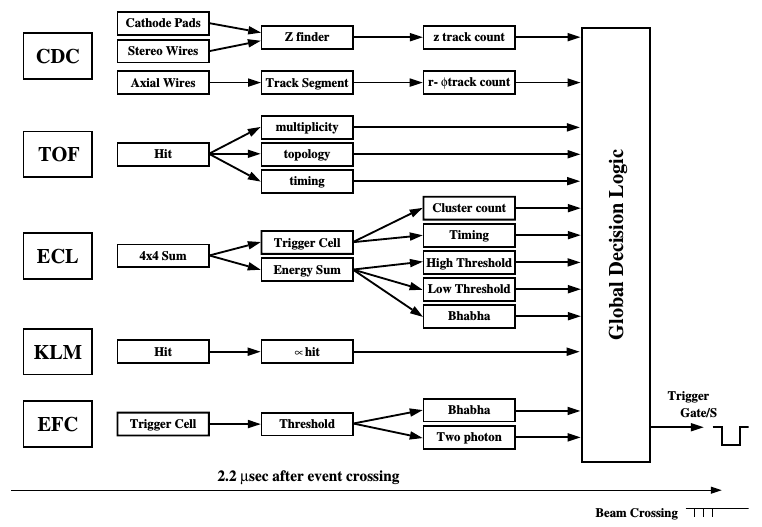
\includegraphics[width=0.8\textwidth]{triggerL1}
  \includegraphics[width=0.8\textwidth]{trig_gscheme_2003}
  \caption{Схема работы аппаратного триггера детектора \belle.}
\label{fig:triggerL1}
\end{figure}

Схема триггерной системы первого уровня приведена на рисунке~\ref{fig:triggerL1}. Эта система состоит из триггерных систем всех подсистем детектора и центральной триггерной системы, называемой Глобальной Логикой Решений (\gdl).  Триггерные системы поддетекторов можно разделить на две группы: триггеры, основанные на регистрации треков, и триггеры, основанные на измерении энергии.  

Триггеры первой группы передают:
\begin{enumerate}
 \item Сигналы сработавших проволочек в \cdc в \rphi- и $z$-направлениях;
 \item Сигналы из \tof, включающая временные измерения и информацию о количестве заряженных частиц в событии и их расположении в пространстве;
 \item Сигналы от мюонной системы о $\mu$-кандидатах.
\end{enumerate}
Триггеры второй группы передают:
\begin{enumerate}
 \item Сигналы из \ecl, соответствующие разным типам адронных событий, основанные на измерении энерговыделения в кристаллах и анализа кластеров;
 \item Специальные сигналы из \ecl и \efc для двухфотонных событий и Баба-рассеяния.
\end{enumerate}
\gdl производит параллельную обработку сигналов с подсистем детектора за $1.85\mus$ и выдает триггерное решение через $2.2\mus$ после взаимодействия пучков.  \gdl имеет четыре триггерных признака для адронных событий:
\begin{enumerate}
 \item Двухтрековый триггер;
 \item Трехтрековый триггер;
 \item Триггер по изолированному кластеру;
 \item Триггер по полному энерговыделению.
\end{enumerate}
Комбинируя эти признаки, \gdl достигает эффективность, превышающую $99\%$ для адронных событий.

\daq собирает информацию со всех подсистем детектора для событий, прошедших аппаратный триггер.  Схема работы \daq приведена на рисунке~\ref{fig:daq}.  Характерный размер адронного события составляет приблизительно~$30~\textrm{кБ}$, что соответствует передаче данных со скоростью~$15~\textrm{МБ/с}$.

\begin{figure}[htb]
 \centering
% \includegraphics[width=0.8\textwidth]{daq-over-bw}daq-overview
  \includegraphics[width=0.8\textwidth]{daq-overview}
  \caption{Схема системы сбора данных детектора \belle~\cite{BelleNIM}.}
\label{fig:daq}
\end{figure}

Программный триггер реального времени использует алгоритмы быстрой реконструкции треков.  Для отбраковки фоновых событий, например, обусловленных пучковым фоном, требуется, чтобы событие содержало треки с продольным прицельным параметром относительно точки взаимодействия $|dz|$ меньше~$5\cm$.  Это требование позволяет уменьшить поток данных на два порядка, сохранив эффективность отбора адронных событий больше $99\%$.

Программный триггер обрабатывает набранные данные и отбраковывает часть из них, накладывая набор минимальных критериев отбора, таких как ограничение прицельного параметра и установление порога энерговыделения.  На этом этапе полностью реконструированные события сохраняются в формате, пригодном для физического анализа.  Определяются, например, импульсы реконструированных заряженных треков, список фотонов из реконструированных кластеров \ecl и информация об идентификации частиц.

Детальное описание триггерной системы и системы сбора данных детектора Belle приведено в работах~\cite{trig,daq1,daq2}.

% [87] Y. Ushiroda, A. Mohapatra, H. Sakamoto et al. “Development of the Central Trigger
% System for the Belle Detector at the KEK B-Factory”. Nuclear Instruments and Methods
% A, 438(2):460–471, 1999.
% [88] S. Y. Suzuki, M. Yamauchi, M. Nakao et al. “The Belle DAQ System”. Nuclear Instru-
% ments and Methods A, 453(1):440–444, 2000.
% [89] S. Y. Suzuki, R. Itoh, H.-W. Kim et al. “Belle DAQ System Upgrade at 2001”. Nuclear
% Instruments and Methods A, 494(1):535–540, 2002.

%\section{Модернизация калориметра детектора Belle} \label{sect3_2}


\section{Модернизация электромагнитного калориметра}\label{sec:ecl-upgrade}
В рамках подготовки эксперимента \belleii~\cite{belleIItdr} на Супер-$B$-фабрике \textrm{SuperKEKB}~\cite{superkekb} ведутся работы по модернизации электромагнитного калориметра детектора Belle.  На начальной стадии, электромагнитный калориметр детектора \belleii будет состоять из $8736$ кристаллов \csit, использовавшихся в эксперименте Belle.  При проектной светимости ускорителя \textrm{SuperKEKB} $8\times 10^{35}\lumi$, фоновая загрузка кристаллов калориметра кардинально увеличится по сравнению с фоновой загрузкой при работе в эксперименте Belle.  Для работы в таких условиях необходимо уменьшить время формирования сигнала и модифицировать считывающую электронику.  

Поставленная задача была решена группой, отвечающей за подготовку калориметра \belleii.  Основным элементом модернизированной системы считывающей электроники \ecl является модуль формирования и оцифровки сигналов (\sdsp).  Каждый \sdsp считывает сигнал с предуселителей $16$-ти кристаллов \csit.  Поступивший в \sdsp сигнал преобразуется с помощью двух фильтров Бесселя и затем оцифровывается с помощью $18$-ти битного аналого-цифрового преобразователя прямого преобразования с тактовой частотой $2~\textrm{~МГц}$ (рисунок~\ref{fig:sdsp}).  Оцифрованный сигнал обрабатывается с помощью аппаратного алгоритма, реализованного в программируемой пользователем вентильной матрице~\cite{fpga1,fpga2}.  % (\fpga).    
Алгоритм возвращает информацию об амплитуде сигнала и времени его прихода относительно триггерного такта и передает ее в систему сбора данных.  Временная информация, которая не была доступна в эксперименте Belle, позволит более эффективно подавлять фоновые срабатывания.  \sdsp также генерирует быстрый аналоговый сигнал для триггерный системы посредством суммирования сигналов со всех $16$-ти входных каналов.  Сигналы складываются с откалиброванными коэффициентами ослабления, обеспечивающими приблизительно одинаковый энергетический порог для каждого канала калориметра.

\begin{figure}[htb]
 \centering
  \includegraphics[width=0.6\textwidth]{sdsp}
  \caption{Схема \sdsp электромагнитного калориметра~\belleii.}
\label{fig:sdsp}
\end{figure}

Для работы калориметра необходимы $576$ \sdsp.  После изготовления модулей необходимо проверить их работоспособность и измерить характеристики.  Для решения этой задачи был создан измерительный стенд, схема которого приведена на рисунке~\ref{fig:testbench}.  

\begin{figure}[H]
 \centering
  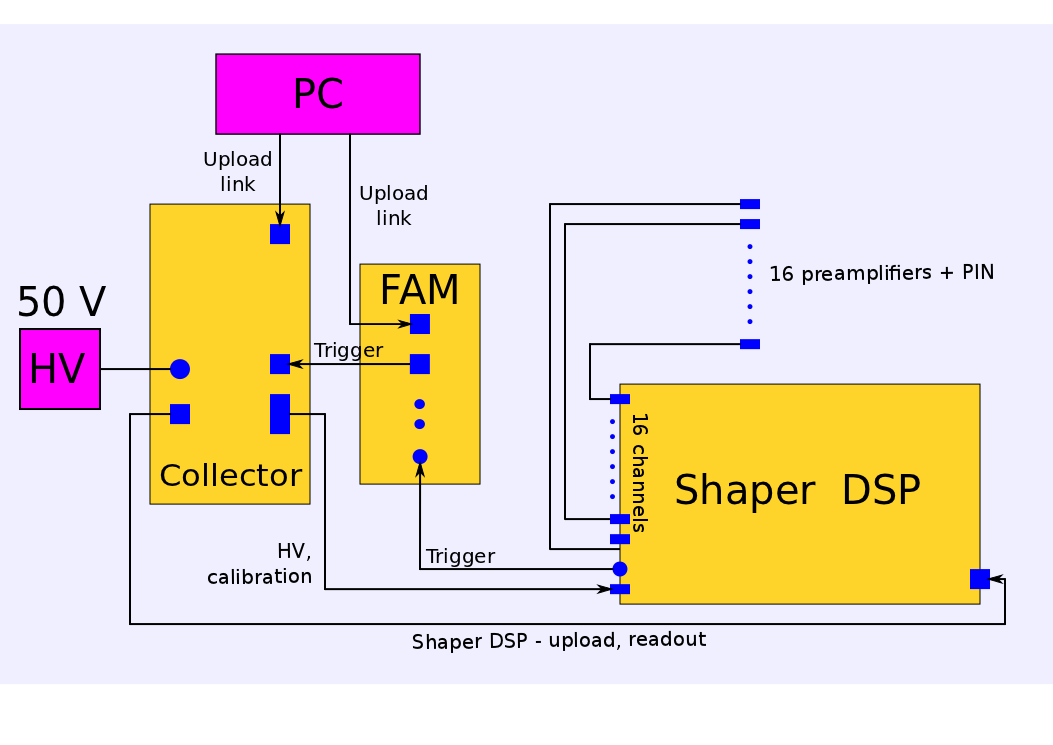
\includegraphics[width=0.7\textwidth]{testbench_scheme}
  \caption{Схема стенда для проверки параметров \sdsp~\cite{testbench}.}
\label{fig:testbench}
\end{figure}

Стенд включает \sdsp, модуль оцифровки быстрого сигнала от \sdsp и коллекторный модуль, принимающий данные об амплитуде и времени сигналов от \sdsp, собранные в стойке VME (VERSAModule Eurocard).  \sdsp может получать входной сигнал либо от $16$-ти предусилителей, установленных на кристаллы \csit, либо калибровочный сигнал, выдаваемый коллекторным модулем.  Оцифрованный сигнал с каждого входного канала \sdsp, оцифрованный быстрый сигнал и данные об амплитуде и времени прихода сигналов передаются в персональный компьютер.

Автором диссертации подготовлено программное обеспечение (ПО) для выполнения автоматической проверки \sdsp на описанном стенде.  Подготовленное ПО использует библиотеки для считывания информации с коллекторного модуля и модуля оцифровки быстрого сигнала, а также для подачи калибровочного сигнала на вход \sdsp.  ПО позволяет в автоматическом режиме выполнять набор и анализ данных, определяя различные характеристики модуля~\cite{testbench}.  

Простой пользовательский интерфейс (рисунок~\ref{fig:testbench-interface}) позволяет использовать ПО, будучи неосведомленным о деталях реализации алгоритмов проверки и взаимодействия с модулями электроники.  Параллельное выполнение набора данных и анализа уже набранных данных (многопоточность) позволило достичь времени выполнения проверки одного \sdsp, приблизительно равного $25$ минутам.  Эта величина определяется в основном временем, необходимым для набора необходимых данных.  Результаты проверки каждого \sdsp и набранные при проверке данные автоматически сохраняются в структурированном виде на носитель информации, что позволяет получать в дальнейшем полную информацию о конкретной проверке и выполнять анализ выполненных проверок.

Автором диссертации реализован один из алгоритмов проверки \sdsp: проверка \emph{линейности} зависимости восстановленной в \sdsp величины амплитуды ($A^{\mathrm{fit}}$) от амплитуды входного сигнала, сформированного коллекторным модулем ($A^{\mathrm{gen}}$), в динамическом диапазоне $5\times10^4$.  В ходе проверки для каждого считывающего канала определяются значения коэффициентов $b$ и $k$, при которых зависимость $A^{\mathrm{fit}} = kA^{\mathrm{gen}} + b$ наилучшим образом описывает полученные данные, а также максимальное относительное отклонение
\begin{equation}
 d = \max\left[\frac{A^{\mathrm{fit}} - \lbr kA^{\mathrm{gen}} + b \rbr}{A^{\mathrm{fit}}}\right].
\end{equation}
На рисунке~\ref{fig:testbench-linearity} приведены распределения по параметрам $k$ и $d$ для $348$ проверенных \sdsp.

\begin{figure}[H]
 \centering
 \begin{minipage}[b]{0.49\textwidth}
 \centering
  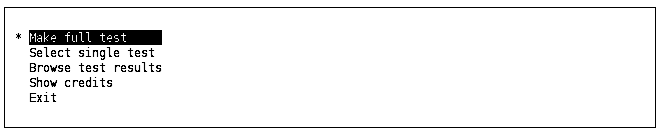
\includegraphics[width=\textwidth]{testbench_main_window_short_v2}
  \subcaption{}
  \label{fig:testbench-main-menu}
 \end{minipage}
 \begin{minipage}[b]{0.49\textwidth}
 \centering
  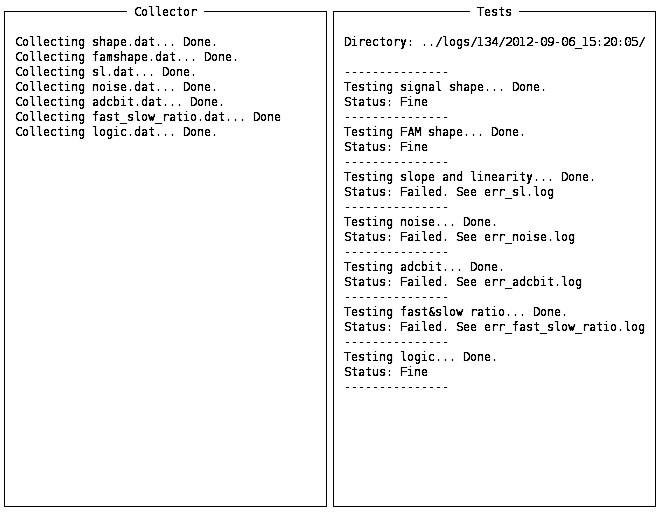
\includegraphics[width=\textwidth]{testbench_collector_and_tests_v2}
  \subcaption{}
  \label{fig:testbench-test-info}
 \end{minipage}
  \caption{Пользовательский интерфейс ПО для тестирования \sdsp: а)~основное меню и б)~пример вывода информации при выполнении автоматической проверки \sdsp.}
\label{fig:testbench-interface}
\end{figure}

\begin{figure}[htb]
 \centering
 \begin{minipage}[b]{0.49\textwidth}
 \centering
  \includegraphics[width=\textwidth]{slope}
  \subcaption{}
  \label{fig:slope}
 \end{minipage}
 \begin{minipage}[b]{0.49\textwidth}
 \centering
  \includegraphics[width=\textwidth]{max_deviation}
  \subcaption{}
  \label{fig:max_deviation}
 \end{minipage}
  \caption{Результаты проверки линейности $348$~\sdsp: а) коэффициент пропорциональности между амплитудой калибровочного сигнала и амплитудой, определенной аппаратным алгоритмом \sdsp и б) максимальное относительное отклонение от линейной зависимости между входной и восстановленной амплитудами.  Гистограммы с наклонной красной и вертикальной синей штриховками соответствуют двум наборам \sdsp, произведенным в разное время.  Незаполненные гистограммы показывают суммарные распределения~\cite{testbench}.}
\label{fig:testbench-linearity}
\end{figure}

Собранная информация о параметрах используемых \sdsp будет использована при выполнении калибровок калориметра.
